\documentclass{standalone}
\usepackage{pgfplots}
\definecolor{darkgreen}{rgb}{0.0, 0.5, 0.0}

\begin{document}
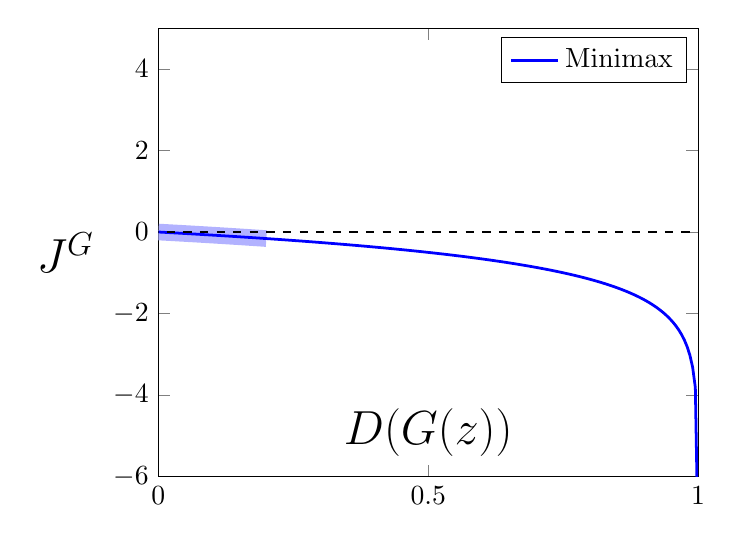
\begin{tikzpicture}
	\begin{axis}[
		xlabel=$D(G(z))$,
		ylabel=$J^G$,
		xmin=0,
		xmax=1,
		ymax=5,
		ymin=-6,
		ylabel near ticks,
		xlabel near ticks,
		xtick={0, 0.5, 1},
		ylabel style={rotate=-90, font=\LARGE},
		xlabel style={font=\LARGE, above=6mm},
	]
	
	% shading
	\addplot[line width=6pt,color = blue!30, domain = 0:0.2, smooth, forget plot]{(1/2) * log2(1-x)};
	
	% use TeX as calculator:
	\addplot [mark=none, domain=0:1, line width=1pt, color=blue, samples=200] {(1/2) * log2(1-x)};
	
	% 0 line
	\addplot[dashed, forget plot]{0};
	
	\legend{Minimax}
	
	\end{axis}
\end{tikzpicture}
\end{document}